% This file was created with tikzplotlib v0.9.17.
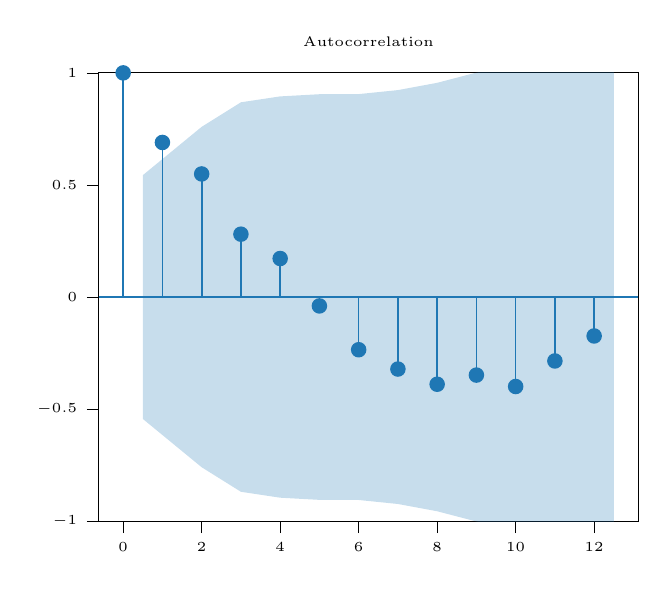
\begin{tikzpicture}

\definecolor{color0}{rgb}{0.12156862745098,0.466666666666667,0.705882352941177}

\begin{axis}[
font={\fontsize{3}{12}\selectfont},
tick align=outside,
tick pos=left,
title={Autocorrelation},
x grid style={white!69.0196078431373!black},
xmin=-0.625, xmax=13.125,
xtick style={color=black},
y grid style={white!69.0196078431373!black},
ymin=-1, ymax=1,
ytick style={color=black}
]
\path [fill=color0, fill opacity=0.25]
(axis cs:0.5,0.543596203409375)
--(axis cs:0.5,-0.543596203409375)
--(axis cs:2,-0.759315183323327)
--(axis cs:3,-0.868775963903635)
--(axis cs:4,-0.895112716713709)
--(axis cs:5,-0.904816481581235)
--(axis cs:6,-0.905328876892921)
--(axis cs:7,-0.923184468402576)
--(axis cs:8,-0.955642998829793)
--(axis cs:9,-1.00135008493124)
--(axis cs:10,-1.03649765716604)
--(axis cs:11,-1.08095780944124)
--(axis cs:12.5,-1.10296966394207)
--(axis cs:12.5,1.10296966394207)
--(axis cs:12.5,1.10296966394207)
--(axis cs:11,1.08095780944124)
--(axis cs:10,1.03649765716604)
--(axis cs:9,1.00135008493124)
--(axis cs:8,0.955642998829793)
--(axis cs:7,0.923184468402576)
--(axis cs:6,0.905328876892921)
--(axis cs:5,0.904816481581235)
--(axis cs:4,0.895112716713709)
--(axis cs:3,0.868775963903635)
--(axis cs:2,0.759315183323327)
--(axis cs:0.5,0.543596203409375)
--cycle;

\path [draw=color0, semithick]
(axis cs:0,0)
--(axis cs:0,1);

\path [draw=color0, semithick]
(axis cs:1,0)
--(axis cs:1,0.689620568292931);

\path [draw=color0, semithick]
(axis cs:2,0)
--(axis cs:2,0.549132585047337);

\path [draw=color0, semithick]
(axis cs:3,0)
--(axis cs:3,0.280365962651206);

\path [draw=color0, semithick]
(axis cs:4,0)
--(axis cs:4,0.171912094119453);

\path [draw=color0, semithick]
(axis cs:5,0)
--(axis cs:5,-0.0396157503797431);

\path [draw=color0, semithick]
(axis cs:6,0)
--(axis cs:6,-0.235041621951144);

\path [draw=color0, semithick]
(axis cs:7,0)
--(axis cs:7,-0.321230271057791);

\path [draw=color0, semithick]
(axis cs:8,0)
--(axis cs:8,-0.389040666255731);

\path [draw=color0, semithick]
(axis cs:9,0)
--(axis cs:9,-0.348130536718216);

\path [draw=color0, semithick]
(axis cs:10,0)
--(axis cs:10,-0.39911789720762);

\path [draw=color0, semithick]
(axis cs:11,0)
--(axis cs:11,-0.28520426113107);

\path [draw=color0, semithick]
(axis cs:12,0)
--(axis cs:12,-0.173650205409611);

\addplot [semithick, color0]
table {%
-0.625 -2.22044604925031e-16
13.125 -2.22044604925031e-16
};
\addplot [semithick, color0, mark=*, mark size=2.5, mark options={solid}, only marks]
table {%
0 1
1 0.689620568292931
2 0.549132585047337
3 0.280365962651206
4 0.171912094119453
5 -0.0396157503797431
6 -0.235041621951144
7 -0.321230271057791
8 -0.389040666255731
9 -0.348130536718216
10 -0.39911789720762
11 -0.28520426113107
12 -0.173650205409611
};
\end{axis}

\end{tikzpicture}
